\chapter{Droites, plans}
\label{chapter:Fr_03-linesplanes}

Dans le chapitre précédent, nous avons rappelé l'algèbre et la géométrie des vecteurs de
$\R^2$ et de $\R^3$, puis nous avons généralisé à $\R^n$ les notions d'addition vectorielle,
de multiplication scalaire, de produit scalaire, d'orthogonalité et d'angle entre deux vecteurs.  


Dans ce qui suit, nous considérerons les droites de $\R^2$, ainsi que les droites et les plans de $\R^3$.  
Nous verrons que certaines notions se généralisent facilement
à $\R^n$, mais que d'autres demandent plus de travail pour aboutir à une généralisation convenable. En fait, trouver ce qui est exactement
l'analogue d'une droite ou d'un plan dans $\R^n$ est l'un de nos objectifs dans ce cours.


\section{Description des droites}

Dans $\R^2$ ou $\R^3$, une droite est définie de manière unique simplement en se donnant un point par lequel elle passe et
un vecteur qui lui donne une direction. 
\begin{figure}
\begin{center}
\vglue-.7cm

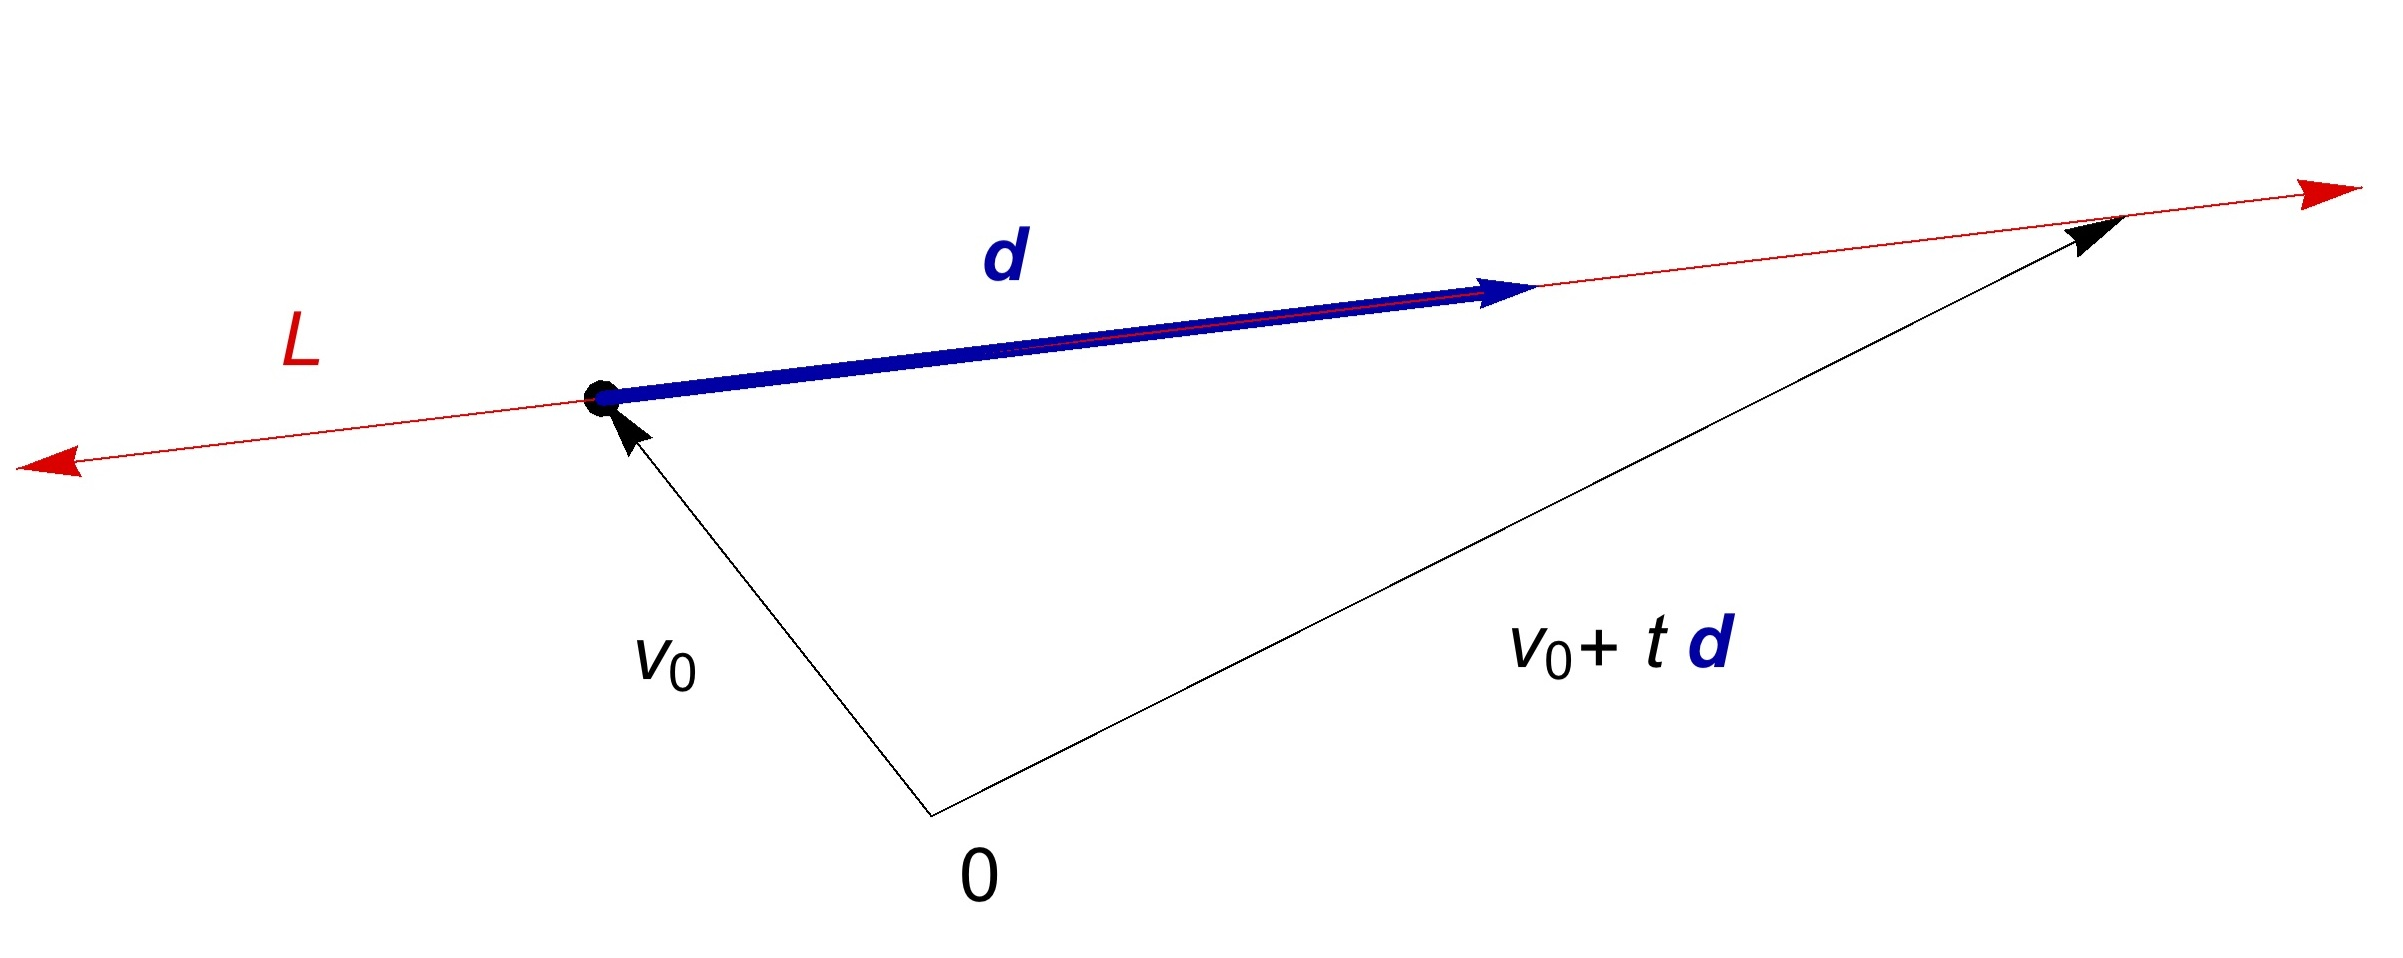
\includegraphics[scale=.1]{linepoint-directionvector.jpg}
\end{center}

\caption{Forme paramétrique vectorielle de $\mathcal L$}\label{vectorparametricformplane}
\end{figure}
Ainsi, la droite $\mathcal L$ passant par le sommet de $\vv_0$ et parallèle à un vecteur $\dd$
est unique et est décrite par l'ensemble
$$
\mathcal L = \{ \vv_0 + t \dd\, |\, t\in \R\}.
$$
En d'autres termes, tout point $\vv$ de la droite $\mathcal L$ peut être écrit comme $\vv = \vv_0+t\dd$ pour un certain $t$. Le vecteur $\dd$ est appelé \defn{vecteur directeur} de $\mathcal L$.

\begin{myexample}
Considérons la droite $y=3x+2$ dans $\R^2$.  Nous pouvons obtenir une équation paramétrique de cette droite en posant $x=t$ comme paramètre et en isolant $y$, et on obtient : 
$x = t$ et $y=3t+2$.  Il est possible de passer à la forme paramétrique vectorielle avec les étapes suivantes :
$$
\mat{x\\y} = \mat{t\\3t+2} = \mat{0+1t\\2+3t} = \mat{0\\2} + t\mat{1\\3}\,.
$$
Ainsi la droite $\mathcal L$ est décrite par
$$
\mathcal L = \left\{ \mat{0\\2} + t\mat{1\\3} \Big| \, t \in \R\right\}.
$$


Remarque : Une autre façon d'obtenir une équation paramétrique de la droite $\mathcal L$ est de prendre deux
points par lesquels elle passe, par exemple $(0,2)$ et $(-\frac{2}{3},0)$, puis de construire le vecteur directeur $\dd$ en calculant la soustraction
$$\dd = \mat{0\\2}-\mat{-2/3\\0} = \mat{2/3\\2}.$$
Maintenant, en prenant par exemple $\vv_0 = (0,2)$, on obtient alors :
$$
\mathcal L = \left\{ \mat{0\\2} + t\mat{2/3\\2} \Big|\, t\in\R\right\}.
$$
Notez qu'on obtient une expression différente de celle qu'on avait précédemment pour $\mathcal L$ : en fait, cette manière d'écrire $\mathcal L$ n'est pas unique car elle dépend de nos choix (on aurait pu plutôt prendre $\vv_0 = (-\frac{2}{3},0)$ par exemple, ou prendre un vecteur $\dd$ deux fois plus grand par exemple). Malgré tout, même si les écritures sont différentes, elle décrivent en fait la même droite $\mathcal L$, et donc plusieurs réponses peuvent être justes (vérifiez ceci avec un dessin !).
\end{myexample}

ATTENTION !  Nous utilisons souvent la variable $t\in\R$ comme paramètre pour une droite, mais si
on veut comparer deux droites différentes, il faut prendre le soin d'utiliser des
lettres différentes, par exemple $t$ et $s$, pour représenter les paramètres dans leurs équations respectives !


\begin{myexample}
Trouvez le point d'intersection (s'il existe) des droites $\mathcal L = \{ t(1,2) \,| \, t \in \R\}$ 
et $\mathcal L' = \{ (0,1)+t(3,0) \,|\, t \in \R\}$.

MAUVAISE M\'ETHODE :  résoudre pour $t$ l'équation vectorielle $t(1,2)=(0,1)+t(3,0)$.
Cette méthode ne donne pas de solution $t$... En fait, ça vient du fait que
les deux droites n'arrivent pas au point d'intersection au même temps $t$. Pourtant, sur un dessin, on voit que ces deux droites se croisent. Elles se croisent donc avec des paramètres $t$ et $s$ différents !


MÉTHODE CORRECTE : Trouver les paramètres $s$ et $t$ tels que
  $t(1,2) = (0,1)+s(3,0)$.  On obtient $t=\frac12$ et $s=\frac16$ et donc le point d'intersection est $(\frac12,1)$. Ouf !
\end{myexample}

Pour une droite de $\R^n$, la forme
$$
\mathcal L = \{ \vv_0 + t \dd~|~ t\in \R\}
$$
 est appelée \defn{forme vectorielle} de $\mathcal L$ ou \defn{forme paramétrique vectorielle} de $\mathcal L$. 
Remarquez que dans $\R^2$, on peut aussi décrire une droite $\mathcal L$ par une équation du type
$ax+by=c$, qu'on appelle \emph{équation cartésienne}\index{equation cartesienne@équation cartésienne} de $\mathcal L$, mais PAS dans $\R^3$ car sinon cette équation décrirait alors un plan !! Voir section \ref{section : description des plans dans R3}.

Notez que la forme paramétrique nous permet aussi d'obtenir des équations paramétriques. Par exemple dans $\R^3$, si l'on se donne $\vv_0 = (a,b,c)$ et $\dd = (d_1,d_2,d_3)$, alors notre droite $\mathcal L$ est l'ensemble de tous les points $\vv=(x_1,x_2,x_3)$ tels que 
\begin{align*}
x_1 &= a+ td_1,\\
x_2 &= b+td_2,\\
x_3 &= c+td_3,
\end{align*}
pour un certain paramètre $t\in \R$.

\section{Remarques sur la géométrie des droites}

Voici quelques observations à propos des droites :
\begin{itemize}
	\item Il n'y a qu'une seule droite dans $\R$: c'est la droite réelle $\R$ elle-même...
	\item Deux droites disjointes dans $\R^2$ peuvent soit être parallèles, soit se croiser en un unique point.
	\item Deux droites disjointes dans $\R^3$ peuvent soit être parallèles, soit se croiser en un unique point, soit être gauches.  Dans les deux premiers cas, elles sont contenues
dans un plan (qui est même unique), mais dans le troisième cas il n'existe pas de plan qui les contient toutes les deux (par contre, on peut trouver deux plans parallèles distincts contenant chacun une des deux droites).
\end{itemize}

\section{Description des plans dans \texorpdfstring{$\R^3$}{R3}}
\label{section : description des plans dans R3}

Rappelez-vous que les plans dans $\R^3$ peuvent être décrits par une équation cartésienne; c'est-à-dire par
l'ensemble des points $(x,y,z)$ tels que
$$
ax+by+cz = d\,,
$$
où $\nn = (a,b,c)$ est un \emph{vecteur normal} au plan,
et où $d\in \R$.

Comment avons-nous obtenu cette équation? 
Si $\vv_0$ est un point quelconque du plan, alors un point $\vv$ appartient au plan ssi $(\vv - \vv_0) \cdot \nn = 0$.  
\begin{figure}
\begin{center}


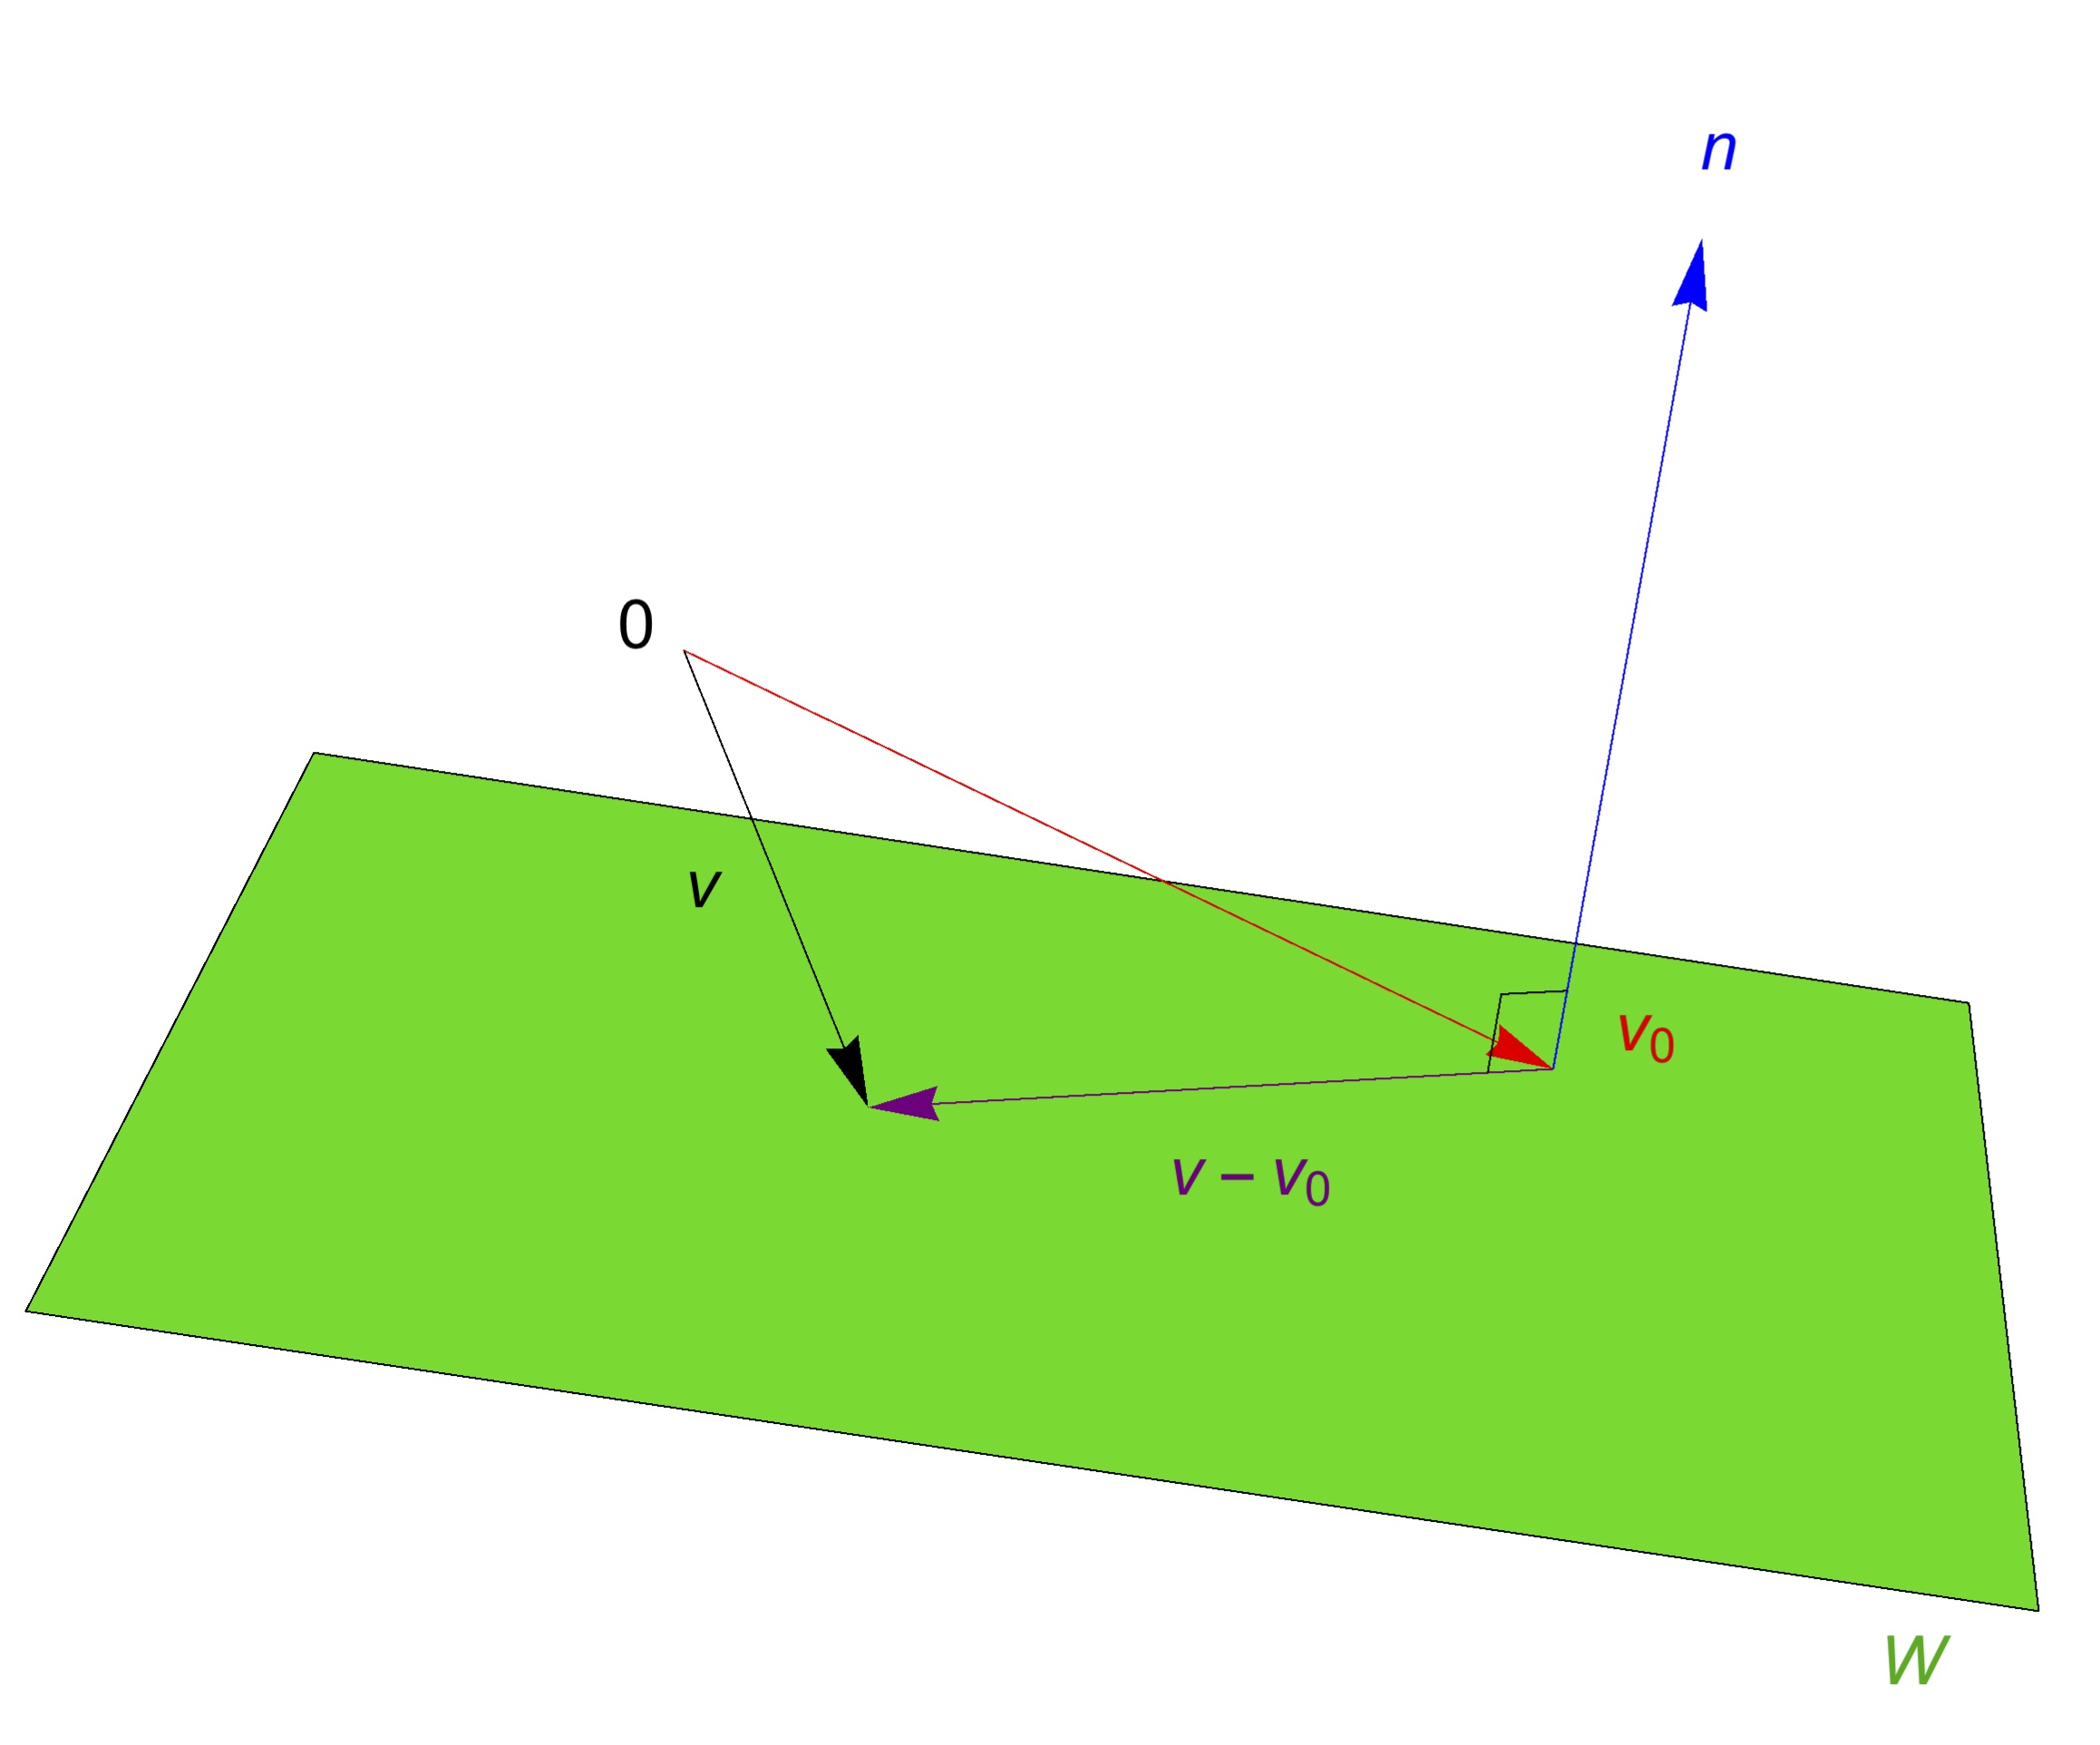
\includegraphics[scale=.087]{cartesianequationplane.jpg}
\end{center}

\caption{\'Equation cartésienne d'un plan}\label{cartesiannormalformalplane}
\end{figure}

Donc le plan passant par $\vv_0$ et de vecteur normal $\nn$ est donné par
$$
\mathcal W = \{ \vv \in \R^3 | (\vv - \vv_0) \cdot \nn = 0 \}.
$$

\begin{myexample}
Le plan passant par $\vv_0 = (1,0,3)$ et de vecteur normal $\nn = (-1,1,2)$
est
\begin{align*}
\mathcal W &= \{ \vv \in \R^3 | (\vv-\vv_0)\cdot \nn=0\}\\
&= \{ (x,y,z) | ((x,y,z)-(1,0,3))\cdot (-1,1,2)=0\}\\
&= \{ (x,y,z) | -(x-1)+(y-0) + 2(z-3) = 0\}\\
&= \{ (x,y,z) | -x+y+2z = 5\}\,.
\end{align*}
(Notez que les coefficients dans l'équation cartésienne nous permettent de retrouver l'expression d'un vecteur normal).
\end{myexample}

Le vecteur normal est utile dans de nombreuses situations. En voici un exemple.

\begin{myprob} 
Trouvez la distance du point $P = (1,2,3)$ au plan $\mathcal W$ d'équation cartésienne $3x-4z=-1$.

\begin{mysol} 


Soit $A$ un point quelconque du plan $\mathcal W$, disons $A=(1,0,1)$, et soit $Q$ le point (inconnu) du plan $\mathcal W$ le plus proche de $P$. En d'autres termes $Q$ est la projection orthogonale\footnote{Voici une preuve. Si $Q'$ est un autre point quelconque sur $\mathcal W$, $\|P-Q'\|^2=\|P-Q+ Q-Q'\|^2= \|P-Q\|^2+ \|Q-Q'\|^2$ (car $P-Q$ et $Q-Q'$ sont perpendiculaires, donc le théorème de Pythagore s'applique). Ainsi $\|P-Q'\|^2\ge \|P-Q\|^2$. } de $P$ sur $\mathcal W$, voir la définition dans la section \ref{section : projection orthogonale sur une droite dans Rn}.
Comme on peut le voir sur la figure ci-dessous, ceci revient à calculer la longueur de la projection du vecteur rouge $\mathbf{PA}=A-P$ sur le vecteur normal $\nn$ en bleu.


\begin{center}

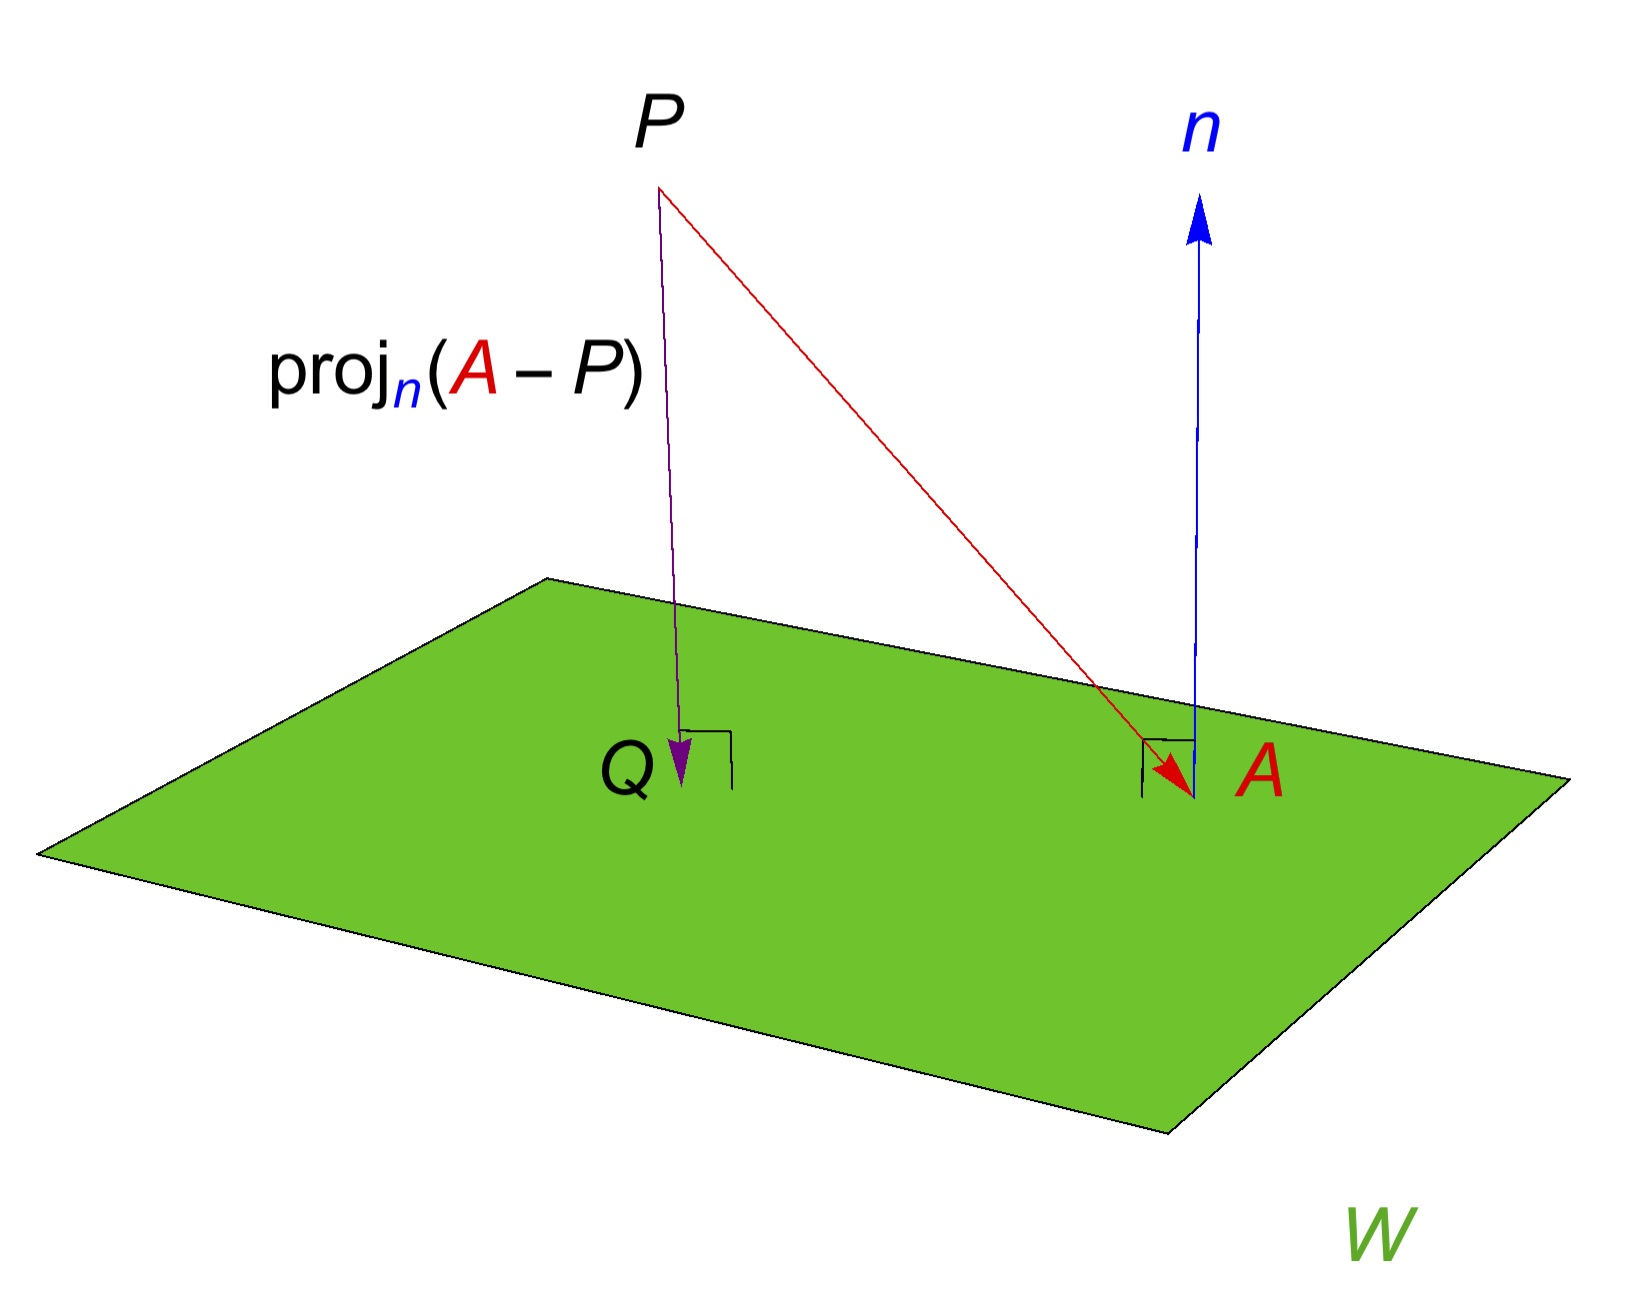
\includegraphics[scale=.4] {projP_on_W.jpg}\\
Distance du point $P$ au plan $\mathcal W$.

\end{center}

On a donc
\begin{align*}
\Vert P-Q \Vert &= \Vert {\proj}_{\nn}(P-A) \Vert\\
&= \Vert {\proj}_{(3,0,-4)}(0,2,2) \Vert\\
&= \Big\Vert \frac{0+0-8}{3^2+(-4)^2}(3,0,-4) \Big\Vert\\
&= \frac{8}{25} \Vert (3,0,-4) \Vert\\
&= \frac{8}{25} \sqrt{25} = \frac{8}{5}.
\end{align*}
\end{mysol}
\end{myprob}

Dans ce qui suit, nous abordons une question plus simple : l'intersection de
deux plans.


\begin{myprob} Trouvez l'intersection des plans $x+y+z = 3$ et $x-y-z=2$.

\begin{mysol} Nous devons trouver tous les points $(x,y,z)$ qui satisfont les deux équations.
Si on soustrait la deuxième équation de la première, on obtient $2y+2z = 1$, ce qui donne $y = \frac12-z$. Alors, à partir de la première équation, nous avons $x = 3-(\frac12-z)-z
= \frac52$.  Mais $z$ peut être arbitraire et donc on peut le considérer comme paramètre (appelons le $t$). On a alors
$$
x = \frac52, \quad y=\frac12-t, \quad z=t
$$
qui est la droite suivante (écrite sous forme vectorielle) :
$$
\mathcal L= \left\{ \mat{5/2\\1/2\\0} + t \mat{0\\-1\\1} | t\in \R\right\}.
$$
\end{mysol}\end{myprob}

\section{Géométrie des plans dans \texorpdfstring{$\R^3$}{R3}}

On définit l'« angle » entre deux plans comme étant l'angle aigu entre deux de leurs vecteurs normaux  
(bien que prouver que ceci à un sens demande quelques réflexions).

Avant de développer plus, comparons les plans de $\R^2$ avec ceux de $\R^3$ :
 
\begin{itemize}
	\item Le seul plan dans $\R^2$ est... $\R^2$ lui-même !

	\item $\R^3$ admet une infinité de plans, et deux plans disjoints de $\R^3$ peuvent soit être parallèles, soit se couper en une droite.
\end{itemize}

Après ceci, on peut alors se poser des questions sur $\R^4$, n'est-ce pas ?
Ceci dit, nous n'avons pas de bonne façon pour décrire (pour l'instant) un plan dans ${\R^4}$, ni même dans $\R^n$ de manière générale pour tout $n\geq 4$ :
en effet, une équation paramétrique vectorielle en une variable donne une droite; et une équation cartésienne donne un hyperplan de dimension $n-1$...  En fait, les équations cartésiennes donnent des objects différents selon la dimension de $\R^n$:

\begin{center}
\begin{tabular}{cccc}
$n$ & & \'Equation dans $\R^n$& Objet géométrique \\ 
\hline
1 &\hphantom{XX} & $ax=b$ & point \\
2 & & $ax+by=c$ & droite \\
3 & & $ax+by+cz =d$ & plan\\
4 & & $ax_1+bx_2+cx_3+dx_4=e$ & ??
\end{tabular}
\end{center}

L'idée derrière tout ça est qu'une équation réduit le \stress{degré de liberté}
(ou la \defn{dimension}, pour utiliser la terminologie \`a venir), et donc le résultat est toujours un objet
de \stress{dimension $n-1$} appelé un \defn{hyperplan} lorsque $n-1\geq3$.

Voici ce qu'on se dit:  puisque l'intersection non-vide de deux plans disjoints de ${\R^3}$ est une droite, l'intersection non-vide de deux hyperplans disjoints de $\R^4$ devrait donner un plan. Wow !
C'est une idée sur laquelle nous reviendrons dans les prochains chapitres.

Mais pour l'instant, revenons à quelque chose de plus concret, dans $\R^3$,
et regardons comment construire facilement des vecteurs normaux d'un plan.

\section{Produit vectoriel dans \texorpdfstring{$\R^3$}{R3}}

Tout d'abord, on adopte la notation suivante :
$$
\hat{i} = \mat{1\\0\\0}, \quad \hat{j} = \mat{0\\1\\0}, \quad \hat{k} = \mat{0\\0\\1}.
$$
Cette notation est intéressante puisqu'alors $(x,y,z) = x\,\hat{i} + y\,\hat{j} + z\,\hat{k}$.

Dans la suite, nous utiliserons également la notation du \emph{d\'eterminant} qui est très pratique à ce niveau.
Le \defn{produit vectoriel} de $\uu = (x,y,z)$ et $\vv=(x', y', z')$
est le vecteur noté $\uu \times \vv$ et donné par 

\begin{align*}
\uu \times \vv &= \left| \begin{matrix}
\hat{i} & \hat{j} & \hat{k} \\
x & y & z\\
x' & y' & z' \end{matrix} \right|\\
&= \left( yz' - y'z, -(xz' - x'z), xy' - x'y \right) \\
&= \left( \left| \begin{matrix} y & z\\ y' & z' \end{matrix} \right|,
- \left| \begin{matrix} x & z\\ x' & z' \end{matrix} \right|,
\left| \begin{matrix} x & y\\ x' & y' \end{matrix} \right| \right)\,.
\end{align*}

\begin{myprob}
Calculez $(1,2,3)\times(4,5,6)$.

\begin{mysol}  Écrivez ceci comme un déterminant puis développez :
$$
\left| \begin{matrix}
\hat{i} & \hat{j} & \hat{k} \\
1 & 2 & 3\\
4 & 5 & 6 \end{matrix} \right|
= (12-15, -(6-12), 5-8) = (-3,6,-3). 
$$
\end{mysol}\end{myprob}

\begin{myprob} Déterminez $(4,5,6)\times(1,2,3)$.

\begin{mysol} De même que dans l'exercice précédent on a :
$$
\left| \begin{matrix}
\hat{i} & \hat{j} & \hat{k} \\
4 & 5 & 6\\
1 & 2 & 3 \end{matrix} \right|
= (15-12, -(12-6), 8-5) = (3,-6,3)\,,
$$
Notez qu'on a obtenu le vecteur opposé à celui d'avant :  $(4,5,6)\times(1,2,3) = -\,(1,2,3)\times(4,5,6)$. 
\end{mysol}\end{myprob}

Par ailleurs, on remarque que :
$$
(1,2,3)\cdot (3,-6,3) = 3-12+9 = 0, \quad (4,5,6)\cdot (3,-6,3) = 12-30+18=0.
$$
Mais rien de tout cela n'est le fruit du hasard!

\begin{theorem} [Propriétés du produit vectoriel]   \label{theoreme : proprietes du produit vectoriel}
Soient $\uu,\vv,\ww\in \R^3$.  Alors :
\begin{itemize}
\item $\uu \times \vv = -\,\vv \times \uu$;
\item $(\uu \times \vv)\cdot \uu = 0$;
\item $(\uu \times \vv)\cdot \vv = 0$;
\item $(\uu + \vv)\times \ww = \uu \times \ww + \vv \times \ww$;
\item $\Vert \uu \times \vv \Vert = \Vert \uu \Vert \; \Vert \vv \Vert \sin(\theta)$, où $0 \leq \theta \leq \pi$ est l'angle entre $\uu$ et $\vv$.
Il s'agit en fait de l'aire du parallélogramme formé par $\uu$ et $\vv$.
\end{itemize}
Notez qu'en général $\uu \times (\vv \times \ww) \neq (\uu \times \vv) \times \ww$; par exemple : $\hat{i} \times (\hat{k} \times \hat{k}) = \zero$ mais $(\hat{i} \times \hat{k})\times \hat{k} = -\hat{i}$. Par conséquent, 
le produit vectoriel n'est ni commutatif ni associatif. 
\end{theorem}


Ainsi, si deux vecteurs $\uu$ et $\vv$ sont parallèles, alors leur produit vectoriel
est nul.  Sinon, leur produit vectoriel est non-nul, c'est l'un des deux vecteurs orthogonaux à la fois à 
$\uu$ et à $\vv$, de longueur $\Vert \uu \Vert \; \Vert \vv \Vert \sin\theta$, où $\theta$ est l'angle entre $\uu$ et $\vv$.
Le produit vectoriel est utilisé par exemple en physique pour mesurer le moment d'une force (le moment traduit l'aptitude de cette force à faire tourner un système mécanique autour d'un point). Il sert aussi à déterminer le troisième vecteur d'une base de $\R^3$ avec la règle des trois premiers doigts de la main droite. Notez qu'une formule facile à retenir est $\hat{i} \times \hat{j} = \hat{k}$ et ses permutations cycliques.

\section[Application: les vecteurs normaux]{Première application du produit vectoriel : Les vecteurs normaux}

Le produit vectoriel donne un vecteur normal aux plans définis par $\uu$ et $\vv$.

\begin{myprob}
Trouvez l'équation du plan contenant les trois points $A = (1,2,3)$,
$B = (1,0,0)$ et $C = (0,1,1)$.

\begin{mysol}
Les vecteurs $\mathbf{BA} = (0,2,3)$ et $\mathbf{BC} = (-1,1,1)$ sont tous les deux
parallèles au plan passant par $A,B,C$, donc tout vecteur $\nn$ normal au plan doit être orthogonal à chacun des deux vecteurs, et la réciproque est aussi vraie. Par le théorème \ref{theoreme : proprietes du produit vectoriel}, on peut donc prendre le produit vectoriel des deux vecteurs :
$$
\nn
=
\mathbf{BA} \times \mathbf{BC}
=
 \left| \begin{matrix}
\hat{i} & \hat{j} & \hat{k} \\
0 & 2 & 3\\
-1 & 1 & 1 \end{matrix} \right| = (-1, -3, 2)\,.
$$
(Vérifiez votre réponse!  Ce vecteur $\nn$ devrait être orthogonal à $\mathbf{BA}$ et à $\mathbf{BC}$.)

L'équation du plan a donc la forme suivante :
$$
-x -3y + 2z = d\,.
$$
Enfin, pour trouver $d$, on utilise un point du plan, disons $B= (1,0,0)$, et on obtient $d=-1$.
\end{mysol} \end{myprob}

\section[Application: volume d'un parallélépipède]{Deuxième application du produit vectoriel : volumes d'un parallélépipède (produit mixte)}

\begin{theorem} [Volume d'un parallélépipède]
Le volume du parallélépipède dont les côtés sont les vecteurs $\uu$, $\vv$ et $\ww$
de $\R^3$ est
$$
\vert (\uu \times \vv) \cdot \ww \vert. 
$$
Notez que l'ordre des vecteurs n'a pas d'importance.
\end{theorem}

Nous pouvons le prouver en utilisant davantage de trigonométrie. Le volume
du parallélépipède est l'aire de la base (un parallélogramme)
fois sa hauteur. Cependant, l'aire de la base est la norme du produit vectoriel
de deux des vecteurs ($\Vert \uu \times \vv \Vert$) et sa hauteur sera de 
$\Vert \ww \Vert \cos(\theta)$, où $\theta$ est l'angle entre
$\ww$ et un vecteur normal à la base.

\begin{myprob}
Trouvez le volume du parallélépipède dont les côtés sont $\uu = (1,0,1)$,
$\vv = (1,2,2)$ et $\ww = (10,0,0)$.

\begin{mysol}
On a
$$
\uu \times \vv =  \left| \begin{matrix}
\hat{i} & \hat{j} & \hat{k} \\
1 & 0 & 1\\
1 & 2 & 2 \end{matrix} \right| 
= (-2,-1,2)
$$
et donc
$$
(\uu \times \vv)\cdot \ww = (-2,-1,2)\cdot (10,0,0) = -20\,.
$$
D'o\`u le volume est de $20$.
\end{mysol}\end{myprob}

Et quelle déduction peut-on faire si l'on a l'égalité $(\uu \times \vv)\cdot \ww = 0$ ?  
On aurait donc un parallélépipède de volume nul, ce qui signifie que ce n'est pas vraiment un parallélépipède...
En fait, cette égalité signifie que les trois vecteurs se trouvent tous dans le même plan. Nous
dirons que ces vecteurs sont \defn{coplanaires}, puisque contenus dans le même plan, et \emph{linéairement dépendants} (terminologie clé pour la suite), puisqu'on peut exprimer un vecteur en fonction des autres.





\section[Remarques finales: les droites, les plans, et plus encore]{Remarques finales sur les droites, les plans et les objets de dimensions supérieures dans \texorpdfstring{$\R^n$}{Rn}}

Faisons quelques réflexions sur certaines idées
que nous explorerons aux prochains chapitres.  Nous avons introduit
des bons moyens d'exprimer les droites et les plans dans $\R^2$ et $\R^3$ : équations paramétriques et équations cartésiennes. Cependant, dans $\R^4$, ces deux techniques échouent pour décrire un objet «~bi-dimensionnel~» alors que notre intuition nous amène à penser qu'ils existent bel et bien.

Ou bien, peut-être pouvons-nous généraliser les procédés des petites dimensions aux grandes dimensions ?\!?

Pour rappel, pour obtenir une droite, nous avons vu qu'il suffit d'avoir un seul paramètre (un degré de liberté): 
$$
\mathcal L = \{ \vv_0+ t\dd_1 \,|\, t\in\R\}\,.
$$
Si maintenant on utilise deux paramètres $s$ et $t$ et deux vecteurs non colinéaires $\dd_1$ et $\dd_2$, on obtient un plan :
$$
\mathcal W = \{ \vv_0 + s\dd_1 + t\dd_2 \,|\, s,t\in\R\}\,.
$$
En d'autres termes, c'est le plan de vecteur normal $\dd_1 \times \dd_2$ et passant par le point $\vv_0$. Ce sera la clé pour généraliser les notions aux dimensions supérieures.

Nous généraliserons prochainement ce type d'énoncé en vue de mieux comprendre les sous-espaces des espaces vectoriels dans le cas général.



